\documentclass[10pt,final,a4paper,oneside,onecolumn]{article}

%%==========================================================================
%% Packages
%%==========================================================================
\usepackage[a4paper,left=3.5cm,right=3.5cm,top=3cm,bottom=3cm]{geometry} %% change page layout; remove for IEEE paper format
\usepackage[T1]{fontenc}                        %% output font encoding for international characters (e.g., accented)
\usepackage[cmex10]{amsmath}                    %% math typesetting; consider using the [cmex10] option
\usepackage{amssymb}                            %% special (symbol) fonts for math typesetting
\usepackage{amsthm}                             %% theorem styles
\usepackage{dsfont}                             %% double stroke roman fonts: the real numbers R: $\mathds{R}$
\usepackage{mathrsfs}                           %% formal script fonts: the Laplace transform L: $\mathscr{L}$
\usepackage[pdftex]{graphicx}                   %% graphics control; use dvips for TeXify; use pdftex for PDFTeXify
\usepackage{array}                              %% array functionality (array, tabular)
\usepackage{upgreek}                            %% upright Greek letters; add the prefix 'up', e.g. \upphi
\usepackage{stfloats}                           %% improved handling of floats
\usepackage{multirow}                           %% cells spanning multiple rows in tables
\usepackage{fancyhdr}                           %% page headers and footers
\usepackage[official,left]{eurosym}             %% the euro symbol; command: \euro
\usepackage{appendix}                           %% appendix layout
\usepackage{xspace}                             %% add space after macro depending on context
\usepackage{verbatim}                           %% provides the comment environment
\usepackage[dutch,USenglish]{babel}             %% language support
\usepackage{wrapfig}                            %% wrapping text around figures
\usepackage{longtable}                          %% tables spanning multiple pages
\usepackage{pgfplots}                           %% support for TikZ figures (Matlab)
\pgfplotsset{compat=1.14}
\usepackage[breaklinks=true,hidelinks,          %% implement hyperlinks (dvips yields minor problems with breaklinks;
bookmarksnumbered=true]{hyperref}   %% IEEEtran: set bookmarks=false)
%\usepackage[hyphenbreaks]{breakurl}            %% allow line breaks in URLs (don't use with PDFTeX)
\usepackage[style=ieee,doi=false,isbn=false,url=false,date=year,minbibnames=6,maxbibnames=15,backend=biber]{biblatex}
%\renewcommand*{\bibfont}{\footnotesize}
\setlength{\biblabelsep}{\labelsep}
\bibliography{../bib}
\usepackage{csquotes}
\usepackage[capitalize]{cleveref}
\crefname{figure}{Figure}{Figures}

\graphicspath{{figures/}}

%%==========================================================================
%% Define header/title stuff
%%==========================================================================
\newcommand{\progressreportnumber}{1}
\renewcommand{\author}{Erwin de Gelder}
\renewcommand{\date}{22 May, 2018}

%%==========================================================================
%% Fancy headers and footers
%%==========================================================================
\pagestyle{fancy}                                       %% set page style
\fancyhf{}                                              %% clear all header & footer fields
\fancyhead[L]{Summary of PhD Research topic. Start: October 1, 2017.}            %% define headers (LE: left field/even pages, etc.)
\fancyhead[R]{\author}                                  %% similar
\fancyfoot[C]{}                                         %% define footer

\begin{document}

\subsection*{Performance assessment methodology for automated vehicles using real-world driving data}

In recent years, much research has been conducted towards automated vehicles. It is generally accepted that testing of automated vehicles will become more and more important and complex. My PhD research focuses on developing a methodology for the assessment of automated vehicles using real-world driving data.

Instead of naively driving millions of kilometers, a scenario-based assessment approach is used. For this approach, the choice of scenarios is crucial. For my PhD research, a data-driven approach is adopted, see \cref{fig:scheme}. The primary goal of the research is to develop a methodology for the generation of the test cases using the preprocessed data, represented by the green blocks in \cref{fig:scheme}. This is achieved by detecting and parameterizing activities. Using the activities and the static environment, the scenarios can be obtained, after which test cases can be generated for the assessment of the automated vehicle.

First of all, a clear definition of scenario is required to avoid the ambiguity that often arises when talking about \emph{scenarios}. Therefore, my first activity regarding my PhD was to define the notion of \emph{scenario} and related notions \cite{degelder2018ontology}. The plan is to use extend the current work \cite{degelder2018ontology} with an ontology and a case study to make it suitable for a journal publication.

On the one hand, the number of scenarios should be limited such that the test load remains feasible and, on the other hand, the scenarios should cover a large part of the variety of the actual scenarios that can be found in real-world traffic. For this reason, it is important to quantify to what extent the collected scenarios and the test cases are \emph{complete}. In \cref{fig:scheme}, this is indicated by the notion of \emph{completeness}. In the context of driving data, the completeness problem is an open issue, so therefore I am currently focusing on this problem. 

Currently, I work on behalf of the Dutch applied research organization (TNO) at Nanyang Technological University (NTU) in Singapore to establish an assessment framework for automated vehicles that is very similar to the approach presented in \cref{fig:scheme} \cite{ploeg2018cetran}. To this end, I am describing so-called scenario classes, i.e., qualitative descriptions of the different scenarios, that are relevant for the assessment of an automated vehicle. Currently, expert knowledge and literature are used to obtain a list of scenario classes. Future work is to obtain the list of scenario classes and the scenarios with a data-driven approach using real-world driving data. To this end, real-world driving data needs to be acquired and the activity detection, parametrization, and scenario mining need to be automated. Other future work is to automate the generation of test cases using the obtained real-world scenarios, such that the test cases are realistic and reflect the more safety-critical scenarios of real-world traffic.

\begin{figure}[h!]
	\centering
	\tikzstyle{block}=[node distance=5.2em, text width=4.5em, minimum height=7em, align=center, rounded corners=8pt, font=\small]
	\tikzstyle{my brace}=[decorate, decoration={brace, amplitude=10pt}]
	\tikzstyle{horz}=[node distance=2.7em]
	\tikzstyle{vert}=[node distance=4em]
	\begin{tikzpicture}[scale=0.95, every node/.style={transform shape}]
		% Draw the blocks
		\node[block, fill=blue!30](dc){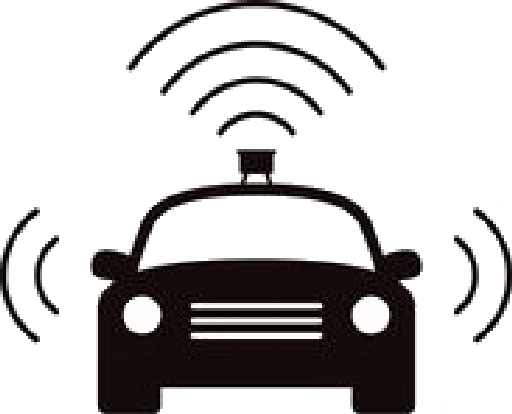
\includegraphics[width=4em]{data_collection.png} \\ Data collection};
		\node[block, fill=blue!30, right of=dc](dp){
\includegraphics[width=2.5em]{data_processing.png} \\ Data preprocessing};
		\node[block, fill=green!30, right of=dp](ed){
\includegraphics[width=4.2em]{event_detection.png} \\ Activity detection};
		\node[block, fill=green!30, right of=ed](p){
\includegraphics[width=3em]{parametrisation.png} \\ Parame-trization};
		\node[block, fill=green!30, right of=p](s){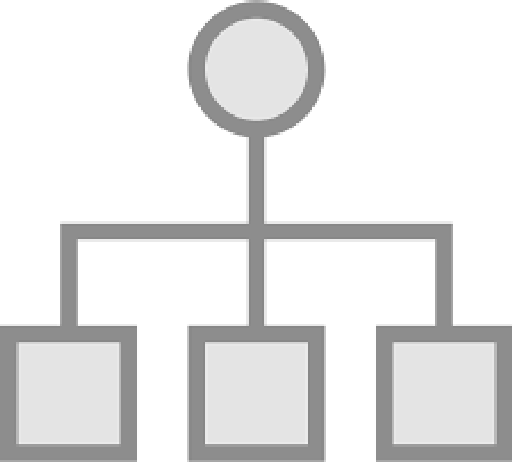
\includegraphics[width=3em]{scenario_mining.png} \\ Scenario mining};
		\node[block, fill=green!30, right of=s](tc){
\includegraphics[width=3.2em]{scenarios.png} \\ Test case genera-tion};
		\node[block, fill=red!30, right of=tc](sim){
\includegraphics[width=4em]{simulation.png} \\ Simulation};
		\node[block, fill=red!30, right of=sim](eval){
\includegraphics[width=3em]{evaluation.png} \\ Evaluation};
		
		% Show completeness part
		\node[horz, left of=ed](b1){};
		\node[vert, below of=b1](b2){};
		\node[horz, right of=tc](b3){};
		\node[vert, below of=b3](b4){};
		\draw[my brace](b4) -- (b2) node[midway, yshift=-2em, align=center]{Completeness};
	\end{tikzpicture}
	\vspace{-1em}
	\caption{Schematic overview of the process of the assessment of an automated vehicle using real-world data. The green blocks are the focus of the PhD research.}
	\label{fig:scheme}
\end{figure}

\vspace{-2em}

\printbibliography

\end{document}